\chapter{FileCatalog connected to a NoSQL database}
One of the main goals of this project was to test whether connecting the 
file catalog, more specifically its metadata part, to a NoSQL database would 
improve the feedback speed of the service thus making it more pleasant to use
or make it easier to implement and maintain. The new database had to satisfy the
following conditions in order to be connectable to DIRAC and deployable in
the computing centers.

\begin{itemize}
\item There has to be a free-ware version which could DIRAC use.
\item The database has to have a python interface or client so it would be easy
to incorporate it into DIRACs code.
\end{itemize}

The characteristics of the data itself add some restrictions. The database should be
optimized for search speed. When combined with the current metaquery implementation, we
get two different types of data retrieval. For directories 
the database has to be able to get all the metadata associated with a directory
identified by an ID. On contrary the files are fetched based on the terms in the metaquery so
all the querying techniques the metaquery could use have to be possible, including
range queries. 

\begin{figure}[h]
\centering
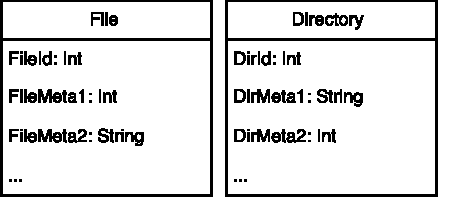
\includegraphics[scale=0.9]{img/dataTyp.pdf}
\caption{Theoretical data scheme in the metadata catalog}
\label{fig:theoDataScheme}
\end{figure}


\section{Apache Cassandra}
Apache Cassandra is a distributed database for managing large amounts of structured data 
across many commodity servers, while providing highly available service and no single point 
of failure \cite{cassandra}. Cassandra's data model is a
partitioned row store, rows are organized into tables. Each row
has an altering number of columns, which are essentially a
key-value pair, and is identified by a unique ID. Adding that Cassandra features
its own query language CQL (Cassandra Query Language) which resembles the standard SQL 
used by all relational databases, it looks like a perfect candidate for the metadata catalog.

\subsection{Developing a data model for Cassandra}

Although CQL makes it look like a relational database, the developer has to bare in mind, that
Cassandra is different. The first scheme used the altering number of columns and organized the 
data in tables, where each file or directory had its own row with metanames being the column
names and values being the column values (this model greatly resembles the theoretical data 
scheme in figure \ref{fig:theoDataScheme}) with secondary indexes over column values so that 
the query would be possible. Although the similarity with SQL would suggest otherwise, 
it turned out that this kind of indexing does not support range queries. 

After understanding more thoroughly how Cassandra works, another data model was introduced 
using most of Cassandras specific features. The key properties Cassandra guaranties are that 
rows are not divided across multiple nodes in the cluster and column keys inside the row
are sorted. Based on these two main characteristics a functioning data model was created. For  
directories row IDs are mapped on directory IDs and the model is similar to the previous one. 
Retrieving a row with given row ID is one of natively supported operations.
For files each metaname has its row, column names are meta values and column values are sets of 
file IDs of files having this metaname and value associated with them. 

\begin{table}[h]
\centering
\label{tab:fileMeta}
\begin{tabular}{|l|l|l|l|ll}
\hline
\multirow{2}{*}{Metaname A} & Value 1      & Value 2      & Value 3      & \multicolumn{1}{l|}{Value 4}      & \multicolumn{1}{l|}{Value 5}      \\ \cline{2-6}
                            & \{id,id,..\} & \{id,id,..\} & \{id,id,..\} & \multicolumn{1}{l|}{\{id,id,..\}} & \multicolumn{1}{l|}{\{id,id,..\}} \\ \hline
\multirow{2}{*}{Metaname B} & Value 1      & Value 2      & Value 3      &                                   &                                   \\ \cline{2-4}
                            & \{id,id,..\} & \{id,id,..\} & \{id,id,..\} &                                   &                                   \\ \cline{1-4}
\end{tabular}
\caption{File metadata}
\end{table}

The rows are grouped
in tables by value type, because the algorithm used to sort the
column names is unified per table. There also is an index over fileID sets, 
so that retrieving all metadata for one specific file is possible, but the scheme is 
not optimized for this operation.

\begin{listing}
\begin{minted}{sql}
CREATE TABLE file_int (
    metaname text,
    value int,
    fileid set<int>,
    PRIMARY KEY (metaname, value)
);
\end{minted}
\caption{Data structure described using CQL}
\end{listing}

In CQL this structure looks like a table with three columns and a compound primary key which
brings the main disadvantage of this approach: meta names can be queried only one at a time and
the result has to be then finalized in the DIRACs code.

\begin{listing}
\begin{minted}{sql}
SELECT fileid 
	FROM file_int 
	WHERE metaname='metaInt1' AND value>3;
\end{minted}
\caption{Example query}
\end{listing}

\section{Document databases}

Both following databases are document-oriented and the data scheme is fairly similar in both
of them. A document-oriented database replaces the concept of a \textit{row} from the world of relational 
databases with a more dynamic and versatile \textit{document}. Allowing arrays and embedded documents the 
document-oriented databases provides de-normalization of the data and represention of complex 
relationships in a single document. Also there are no predefined schemas, which helps with development 
and testing and in case of this project is essential because the number of associated metadata varies between 
files. The metadata are stored in a JSON structure with fields being meta names, indexes above properties and key 
mapped to the dir or file ID.

\begin{listing}
\begin{minted}{json}
{
	'id'       : id
	'metaInt1' : 1,
	'metaStr1' : 'qwerty',
	'metaInt3' : 123
}
\end{minted}
\caption{JSON structure used in document databases}
\end{listing}

Document databases were not the first pick during developing this project, because the idea of
storing metadata in a JSON structure and then building indexes above the properties is not as
familiar as Cassandras columns, but it turned out to be even easier to use.

\subsection{MongoDB}

Mongo is a open-source document-oriented database storing JSON files. As of October 2015, MongoDB is the fourth 
most popular type of database management system, and the most popular for document stores 
\footnote{Ranking database management systems according to their popularity: \url{http://db-engines.com/en/ranking}, ref. October 2015}. 
In MongoDB the document is the basic unit, documents are grouped into collections, which can be thought of as 
a table with a dynamic schema. Single instance of MongoDB can have multiple databases, each can host multiple 
collections. In collections documents are identified using a special field \texttt{\_id} which has to be unique
within a collection (this projects maps the file or directory ids from the file catalog to this id field) \cite{MongoBook}.

\subsubsection{Using MongoDB}

Running MongoDB is rather simple: on Scientific Linux it could be installed from a package with reasonable 
defaults (the only thing that was changed on the testing server was the data directory and listening on the 
universal IP address had to be enabled, default is only local host). %TODO finish

\subsection{Elasticsearch}

Elasticsearch (ES) is a real-time distributed opend-source analytics and search engine \cite{ESBook}, 
build on top of Apache Lucene\footnote{\url{https://lucene.apache.org/}}. Unlike very complex Lucern, 
ES features a simple RESTful API. Moreover it could be used not only for full-text search, but for real-time
analytics or, which is important for this project, as a distributed document store, where \textit{every} field
is indexed and search-able. Its' python 
client\footnote{\url{http://elasticsearch-py.readthedocs.org/en/master/}} provides a wrapper for the RESTful API
as well as some useful additional commands called helpers (e.g. for loading the data, the command 
\texttt{helpers.bulk(es, dataToLoad(size))} was used).

\subsubsection{Using ES}

As well as MongoDB, Elasticsearch ships in a package so downloading and installing it is very simple. The 
configuration file is in \texttt{yaml} format. There is no need for any initial data structure,
the first data are simply inserted using the correct URL\footnote{\url{http://host:port/index/doc_type/doc_id}
is the URL the RESTful API uses, when using the python library \texttt{index, doc\_type}\texttt{doc\_id} are 
specified using the function arguments}. ES structures data in indexes and types (hence the \texttt{index} and
\texttt{doc\_type} in the URL). An Elasticsearch cluster can contain multiple indexes, which can contain multiple
types (there is a rough parallel with the world of relational databases, where indexes would be databases and
types would correspond with tables). Unlike the relational databases ES can create the index and type with the 
first inserted document using its' default configuration.

\section{Database tests}

For testing a single server was used (formerly in one of the Tier-2 computing centers, equipped
%TODO parametry storje puppet2 )
The testing data was generated trying to copy the production data structure. There is expected to
be over 10 million files with approximately different 20 meta names. %TODO odkaz na prilohu s Jirkovym mailem 
The set generated had $10 000 000 - 1$ files with $1$ to $998$ metrics associated with them 
(the generator chose a randomly $1$ to $499$ integer metrics and the same number of string ones).
The metrics names were \texttt{test[Int|Str]NNN}, where \texttt{NNN} stands for a number. The
integer values were all picked from the interval $[1;1000]$ and the string values were one of the
words from the NATO phonetic alphabet %TODO citace.
This lead to the easier composition of testing queries.

The data in form of two csv files with lines \texttt{id,metaname,value} were 63 and 59 GB big.

\subsection{Loading the big data}

Elasticsearchs python interface features a bulk load function which when fed with a generator
loads the data in chunks of 500. Unfortunately it crashes on a TimeoutException from time to 
time making the loading a rather long procedure. 

MongoDB features a command \texttt{mongoimport} which can read a file of JSON objects and load
them all. Its' pace on the test data was approximately $150-200$ entries per second. Unluckily 
the script froze from time to time so loading the whole dataset took again several days.
